\documentclass[aspectratio=169]{beamer}

% Use metropolitan theme
\usetheme{metropolis}

% Packages
\usepackage{booktabs}
\usepackage{colortbl}

% Title page information
\title{Empirical Pricing Factors in Theoretical Economies}

\author{Kerry Back \and Alexander Ober \and Seth Pruitt}


\date{}

% Footer setup
\setbeamertemplate{frame numbering}[fraction]
\setbeamertemplate{footline}{
  \begin{beamercolorbox}[wd=\textwidth,ht=3ex,dp=1.5ex,leftskip=0.3cm,rightskip=0.3cm]{structure}
    Rice Brown Bag, 12/16/2025
    \hfill
    \insertframenumber{} / \inserttotalframenumber
  \end{beamercolorbox}
}

\begin{document}

% Title slide
\begin{frame}
  \titlepage
\end{frame}

% Overview slide
\begin{frame}{Overview}

  \begin{itemize}
    \item Large literature documents relations between characteristics and returns in rational theoretical models.
    \item Pricing is by unobservable (latent) SDF.  SDF betas are correlated with characteristics.
    \item What is the best way to uncover the observable (tradable) SDF?
  \end{itemize}
\pause
\vspace{0.1cm}

Theoretical models: Berk-Green-Naik (1999), Kogan-Papanikolaou (2014), Gomes-Schmid (2021)
\pause
\vspace{0.3cm}

Empirical methods: Fama-French, Fama-MacBeth (\& Rosenberg), Didisheim-Ke-Kelly-Malamud (Complexity)
\end{frame}


\begin{frame}[c]
  \centering
  \Huge Empirical Methods
\end{frame}


\begin{frame}{Empirical Approach}
Define factor weights by some recipe as functions of cross-section of characteristics.

\vspace{0.5cm}
Examples: Fama-French, Fama-MacBeth-Rosenberg, DKKM
\end{frame}


\begin{frame}{Didisheim-Ke-Kelly-Malamud, 2023:  Random Fourier Features}

\begin{itemize}
  \item Factors = returns of portfolios whose weights are rank-standardized characteristic values in $[-0.5, 0.5]$
 \begin{itemize}
  \item Example: book-to-market factor would be return of portfolio that is long value stocks (above median bm) and short growth stocks (below median bm).
  \item "More value" $\Rightarrow$ higher weight.  "More growth" $\Rightarrow$ more negative weight.
  \end{itemize}
  \pause
  \item Start with $M$ characteristics $c_{ik}$.  Generate $M$ random numbers $h_k$.  Compute two new composite characteristics
$$\cos\left(\sum_{k=1}^M h_kc_{ik}\right) \quad \text{and} \quad \sin\left(\sum_{k=1}^M h_kc_{ik}\right)$$
\pause
  \item Repeat many times to get thousands of new composite characteristics.
  \item Define a factor as described before for each of the new composite characteristics
\end{itemize}
\end{frame}

\begin{frame}{DKKM Empirical Results}
\begin{itemize}
  \item 130 stock characteristics
  \item Out-of-sample Sharpe ratios reach 4.0 with high-complexity models (10,000+ factors)
   \item Fama-French-Carhart 6-factor Sharpe ratio $\approx$ 1.1
 \end{itemize}
\end{frame}

\begin{frame}[c]
  \centering
  \Huge Data-Generating Models
\end{frame}

\begin{frame}{Theoretical Models: Overview}
\begin{itemize}
\item In all models, risk premia depend on covariances with a stochastic discount factor.
\item In all models, the covariances are correlated in the cross-section with firm characteristics.
\item Hence, characteristics `explain' risk premia.
\item In all models, we can compute size, book-to-market, profitability, asset growth, and momentum (the FFC6 characteristics).
\item We can also compute the true traded stochastic discount factor and the true tangency portfolio.
\end{itemize}
\end{frame}

\begin{frame}{Berk, Green, and Naik (1999)}
\begin{itemize}
  \item Firms invest optimally given an exogenous pricing kernel
  \item Fixed number of firms, each receives take-it-or-leave-it investment opportunities each period
  \item Projects generate operating cash flows until they randomly die
  \item Investment depends on project NPV (which varies with beta and interest rates)
  \item Model generates: book value, market value, net income, stock returns
  \item Characteristics: size, book-to-market, ROE, asset growth, momentum
\end{itemize}
\end{frame}

\begin{frame}{Kogan and Papanikolaou (2014)}
\begin{itemize}
  \item Firms invest optimally given an exogenous pricing kernel
  \item Two aggregate state variables:
  \begin{itemize}
    \item Disembodied productivity affecting all capital
    \item Productivity of newly installed capital
  \end{itemize}
  \item Firms acquire projects stochastically at firm-specific rates
  \item Optimal capital investment choice for each project
  \item Firm-specific and project-specific productivity processes
  \item Projects produce cash flows until they randomly expire
\end{itemize}
\end{frame}

\begin{frame}{Gomes and Schmid (2021)}
\begin{itemize}
  \item General equilibrium model with heterogeneous firms
  \item Representative household with Epstein-Zin preferences (endogenous SDF)
  \item Firms make optimal investment and financing decisions
  \item Single aggregate productivity process (AR(1)) + firm-specific shocks
  \item Stochastic investment opportunities with random costs
  \item Lumpy investment (discrete project adoption)
  \item Debt: consol bonds paying coupons until random expiration
  \item Tax benefits of debt; costly equity issuance (pecking order)
  \item Strategic default when equity value $\leq 0$
\end{itemize}
\end{frame}


\begin{frame}[c]
  \centering
  \Huge Our Simulations
\end{frame}

\begin{frame}{Motivation for Simulations}
\begin{itemize}
\item In data-generating models, true betas with respect to the SDF depend on entire history of firm-specific and macro shocks
\item Characteristics-based factor models use observable firm characteristics to construct traded factors
\item Betas with respect to these factors partially explain risk premia
\item Our questions: For a given set of characteristics, what is the best way to construct traded factors?  Is the answer robust across models?
\end{itemize}
\end{frame}

\begin{frame}{Simulation Design}
\begin{itemize}
  \item 1,000 firms and 920 months in each panel (discard first 200 as burn-in, leaving 60 years)
  \item 9--12 independent panels for each data-generating model
  \item In each panel for each model in each month, compute true conditional SDF and true conditional max Sharpe ratio
  \item Use calibrations from original papers, except we substitute exogenous lognormal SDF in GS, calibrated to match market risk premium
\end{itemize}
\end{frame}


\begin{frame}{Evaluations of Empirical Methods}
Don't use any specific set of test assets.  Instead:
\begin{itemize}
\item Compare conditional max Sharpe ratios of estimated MVE portfolios of factors

\vspace{0.4cm}
\begin{quote}
\leftskip=2em\rightskip=2em
\upshape Barillas-Shanken, 2017: in horse race between factor models, assuming test assets include competing factors, model with highest Sharpe ratio wins
\end{quote}
\item Estimate conditional SDFs implied by the models and compute Hansen-Jagannathan distance to true conditional SDF

\vspace{0.4cm}
\begin{quote}
\leftskip=2em\rightskip=2em
\upshape HJ distance is the maximum pricing error over all test assets with unit uncentered second moment
\end{quote}
\end{itemize}
\end{frame}

\begin{frame}{Britten-Jones Regression}
  \begin{itemize}
\item Can find empirical mean-variance frontier by linear regression of constant 1 on asset excess returns
\item Write fitted regression as
\begin{align*}
1 &=  \sum_{i=1}^N \hat \beta_i (r_{i}-r_{f}) + \hat \varepsilon \\
&= \hat z + \hat \varepsilon
\end{align*}
\item Max Sharpe ratio is $\bar z/ \sigma_z$
\item Result originally due to Hansen and Richard for population: projection in population rather than regression in sample
\end{itemize}
\end{frame}

\begin{frame}{Britten-Jones Regression}
  \centering
  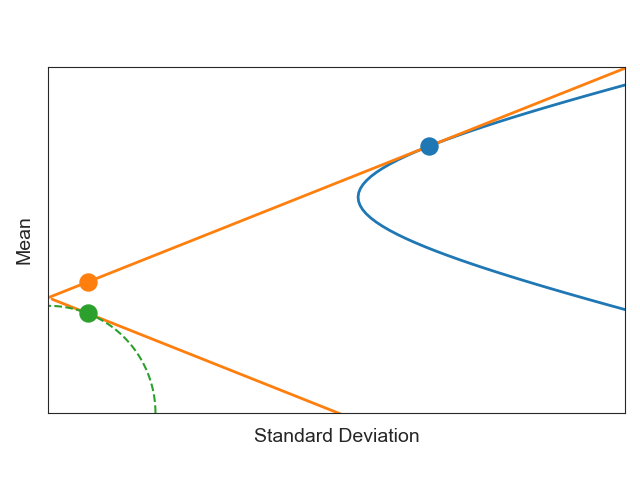
\includegraphics[height=0.6\textheight]{meanvar.png}

\vspace{-0.2cm}
\begin{itemize}
\item Green dot $= (1+r_f) \hat \varepsilon - 1$
\item Orange dot $= r_f + (1+r_f)\hat z$, the Sharpe ratio of which equals $\bar z /\sigma_z$
\item Efficient part of frontier is $\{r_f + b\hat z \mid b \ge 0\}$
\end{itemize}
\end{frame}

\begin{frame}{Our Implementation}
\begin{itemize}
\item Use known true distributions to calculate $\hat \varepsilon$.  Use as SDF (orthogonal to excess returns).
\item In empirical factor models, use Britten-Jones regression on rolling 360 month windows (following DKKM)
\item With many factors (maybe more than 360), use ridge penalization in Britten-Jones regression (following DKKM)
\end{itemize}
\end{frame}

\begin{frame}{Performance Measures for Each Factor Model}
\begin{itemize}
\item Mean theoretical conditional max Sharpe ratio in each panel
\item Realized HJ distance: Square root of mean value of $(\hat \varepsilon_{\text{factors}} - \hat \varepsilon_{\text{all-returns}})^2$ in each panel
\item Both averaged across panels
\end{itemize}
\end{frame}

\begin{frame}{Ridge Regression}
\begin{itemize}
  \item Minimize: $\frac{1}{T}\sum_{t=1}^T (1 - \beta' F_t)^2 + \alpha \beta'\beta$
  \item Penalty parameter $\alpha$ controls shrinkage toward zero
  \item Essential when number of factors $M$ is large relative to sample size $T$
  \item We tune $\alpha$ to optimize performance
\end{itemize}
\end{frame}

\begin{frame}{Empirical Factors}
\begin{itemize}
\item Form factors from size, book-to-market, operating profitability, asset growth, and momentum in all models
\item Fama-French-Carhart (FFC): usual $2\times 3$ sorts, use size/book-to-market sort to form SMB
\item Fama-MacBeth-Rosenberg (FMR): Fama-MacBeth regressions on characteristics
\item Didisheim-Ke-Kelly-Malamud (DKKM): random Fourier features built from the five characteristics plus market return (not penalized in ridge)
\end{itemize}
\end{frame}

\begin{frame}{Fama-MacBeth-Rosenberg}
\begin{itemize}
  \item Fama-MacBeth (1973), Rosenberg (1976), Fama (1976)
  \item Regression coefficients $(X'X)^{-1}X'y$ are linear combinations of returns $y$
  \item Set $W = X(X'X)^{-1}$ so regression coefficients are $W'y$
  \item \# columns $W=$ \# characteristics $+1$
  \item $X'W=I$ implies columns of $X$ and $W$ are orthonormal.
  \item Many solutions $W$ of $X'W=I$, but projection $W=X(X'X)^{-1}$ solves, for each column, $\min \; w'w$ subject to orthonormal constraint
  \item Being orthogonal to column of 1's implies long-minus-short portfolio.  We rescale so long and short sides each sum to 1.
\end{itemize}
\end{frame}


\begin{frame}[c]
  \centering
  \Huge Results
\end{frame}


\begin{frame}{FFC and FMR Perform about the Same}
  \centering
  \begin{tabular}{l c c c c c c c c}
\toprule
& & \multicolumn{3}{c}{Sharpe Ratio} & \multicolumn{3}{c}{HJ Distance} \\
\cmidrule(lr){3-5} \cmidrule(lr){6-8}
Model & SDF & CAPM & FFC & FMR & CAPM & FFC & FMR \\
\midrule
BGN & 0.65 & 0.20 & 0.36 & 0.37 & 0.50 & 0.43 & 0.51 \\
KP14 & 0.24 & 0.12 & 0.19 & 0.18 & 0.23 & 0.19 & 0.20 \\
GS21 & 2.24 & 0.01 & 1.52 & 1.52 & 0.91 & 0.45 & 0.49 \\
\bottomrule
\end{tabular}
\end{frame}

\begin{frame}{DKKM Results}
\begin{itemize}
  \item Performance increases with number of factors (given sufficient penalization)
  \item Best results with 3,600 factors
  \item Optimal $\alpha$:
  \begin{itemize}
    \item BGN: $\alpha = 0.01$
    \item KP14: $\alpha = 0.1$
    \item GS21: $\alpha \approx 10^{-4}$
  \end{itemize}
\end{itemize}
\end{frame}

\begin{frame}{DKKM Sharpe Ratios: BGN Model}
  \centering
  \begin{tabular}{l c c c c}
\toprule
$\alpha$ & 6 & 36 & 360 & 3600 \\
\midrule
0 & 0.400 & 0.405 & 0.019 & 0.189 \\
0.001 & 0.399 & 0.422 & 0.404 & 0.402 \\
0.01 & 0.394 & 0.426 & 0.429 & 0.428 \\
0.05 & 0.379 & 0.410 & 0.414 & 0.414 \\
0.1 & 0.365 & 0.393 & 0.397 & 0.397 \\
1.0 & 0.283 & 0.291 & 0.292 & 0.292 \\
\bottomrule
\end{tabular}
\end{frame}

\begin{frame}{DKKM HJ Distance: BGN Model}
  \centering
  \begin{tabular}{l c c c c}
\toprule
$\alpha$ & 6 & 36 & 360 & 3600 \\
\midrule
0 & 0.407 & 0.439 & 21.959 & 1.563 \\
0.001 & 0.407 & 0.415 & 0.428 & 0.434 \\
0.01 & 0.409 & 0.396 & 0.388 & 0.388 \\
0.05 & 0.417 & 0.398 & 0.393 & 0.393 \\
0.1 & 0.427 & 0.408 & 0.405 & 0.406 \\
1.0 & 0.472 & 0.468 & 0.468 & 0.468 \\
\bottomrule
\end{tabular}
\end{frame}

\begin{frame}{DKKM Sharpe Ratios: KP14 Model}
  \centering
  \begin{tabular}{l c c c c}
\toprule
$\alpha$ & 6 & 36 & 360 & 3600 \\
\midrule
0 & 0.195 & 0.136 & 0.003 & 0.014 \\
0.001 & 0.197 & 0.168 & 0.153 & 0.151 \\
0.01 & 0.202 & 0.195 & 0.193 & 0.192 \\
0.05 & 0.205 & 0.207 & 0.207 & 0.207 \\
0.1 & 0.204 & 0.207 & 0.207 & 0.207 \\
1.0 & 0.180 & 0.184 & 0.184 & 0.183 \\
\bottomrule
\end{tabular}
\end{frame}

\begin{frame}{DKKM HJ Distance: KP14 Model}
  \centering
  \begin{tabular}{l c c c c}
\toprule
$\alpha$ & 6 & 36 & 360 & 3600 \\
\midrule
0 & 0.180 & 0.290 & 20.202 & 1.032 \\
0.001 & 0.178 & 0.223 & 0.250 & 0.254 \\
0.01 & 0.172 & 0.180 & 0.183 & 0.183 \\
0.05 & 0.170 & 0.167 & 0.167 & 0.167 \\
0.1 & 0.171 & 0.167 & 0.167 & 0.167 \\
1.0 & 0.197 & 0.194 & 0.194 & 0.194 \\
\bottomrule
\end{tabular}
\end{frame}

\begin{frame}{DKKM Sharpe Ratios: GS21 Model}
  \centering
  \begin{tabular}{l c c c c}
\toprule
$\alpha$ & 6 & 36 & 360 & 3600 \\
\midrule
0 & 1.634 & 1.828 & 0.194 & 0.223 \\
1e-5 & 1.634 & 1.827 & 1.674 & 1.591 \\
1e-4 & 1.634 & 1.814 & 1.760 & 1.738 \\
5e-4 & 1.634 & 1.789 & 1.777 & 1.772 \\
0.001 & 1.633 & 1.777 & 1.773 & 1.772 \\
0.01 & 1.618 & 1.751 & 1.759 & 1.760 \\
\bottomrule
\end{tabular}
\end{frame}

\begin{frame}{DKKM HJ Distance: GS21 Model}
  \centering
  \begin{tabular}{l c c c c}
\toprule
$\alpha$ & 6 & 36 & 360 & 3600 \\
\midrule
0 & 0.437 & 0.315 & 7.230 & 1.155 \\
1e-5 & 0.438 & 0.317 & 0.363 & 0.397 \\
1e-4 & 0.438 & 0.326 & 0.336 & 0.343 \\
5e-4 & 0.439 & 0.342 & 0.340 & 0.341 \\
0.001 & 0.440 & 0.350 & 0.347 & 0.347 \\
0.01 & 0.454 & 0.380 & 0.375 & 0.375 \\
\bottomrule
\end{tabular}
\end{frame}

\begin{frame}{Sharpe Ratio Distribution: BGN Model}
  \centering
  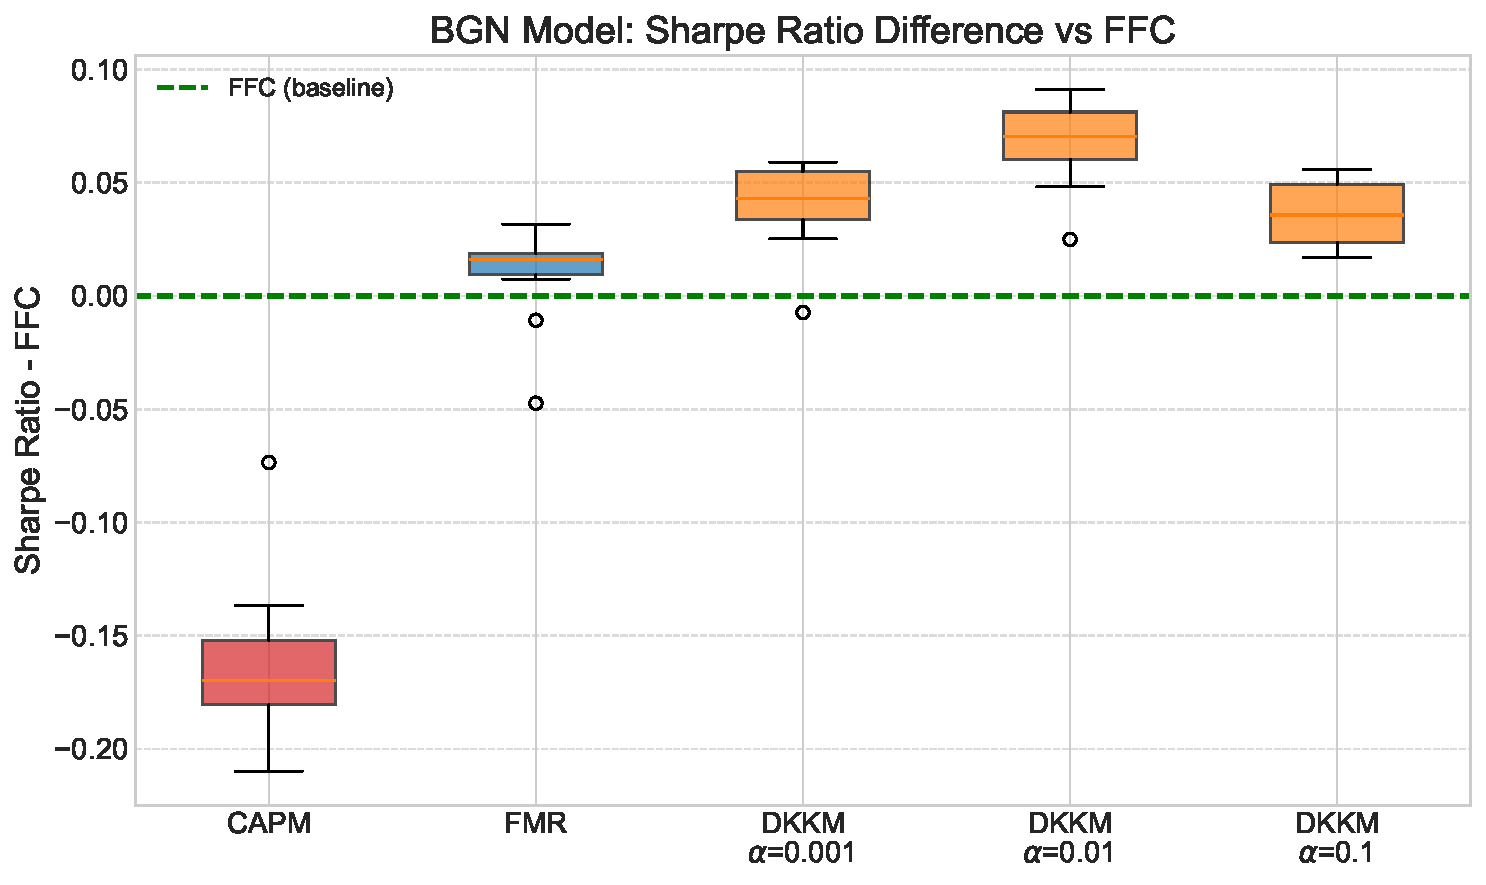
\includegraphics[height=0.85\textheight]{figures/sharpe_boxplot_bgn.pdf}
\end{frame}

\begin{frame}{Sharpe Ratio Distribution: KP14 Model}
  \centering
  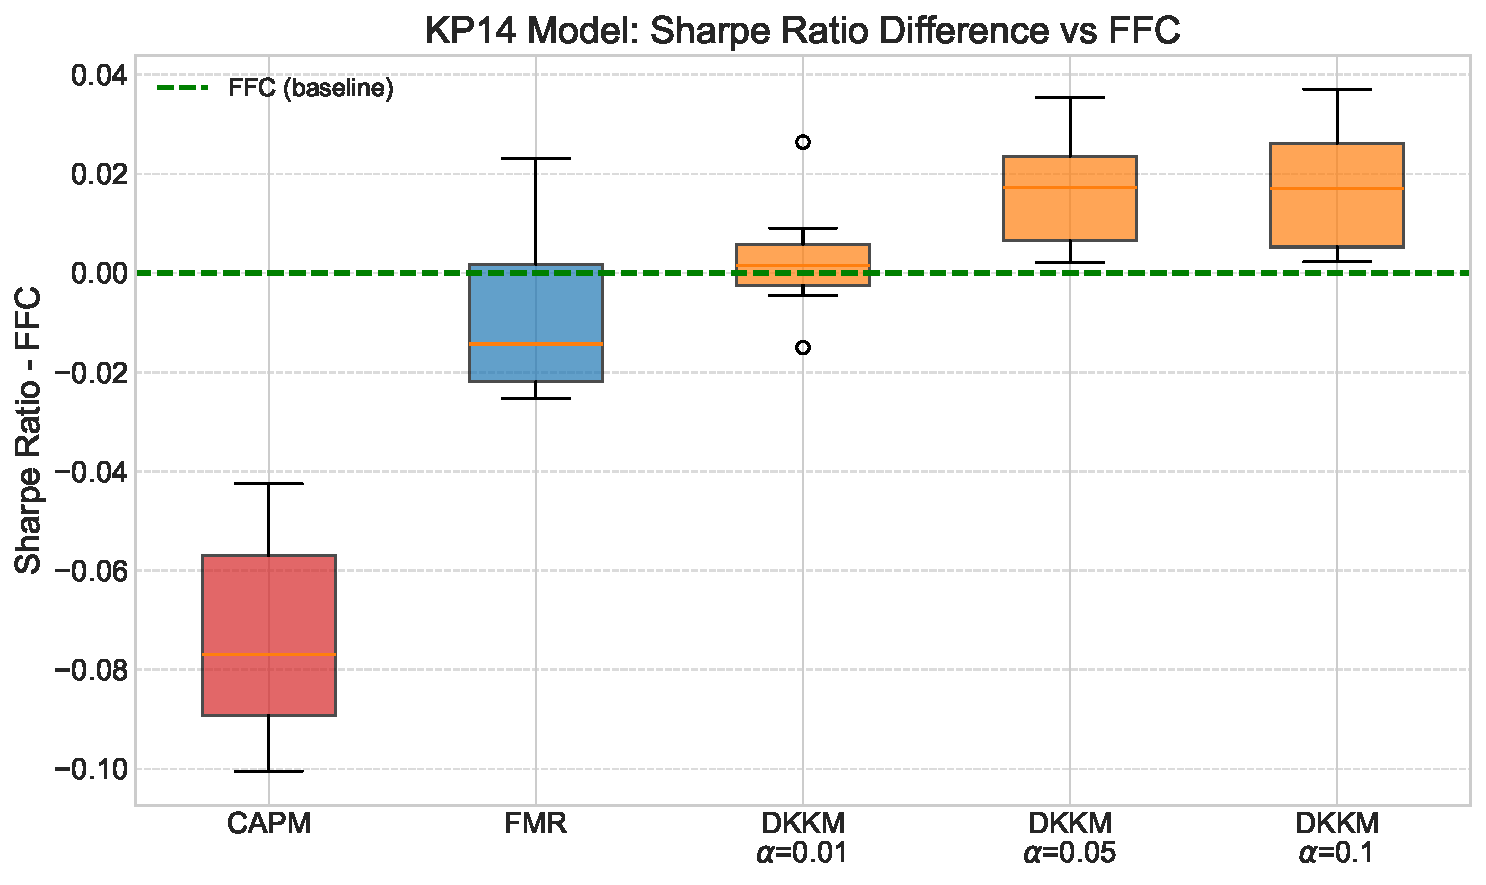
\includegraphics[height=0.85\textheight]{figures/sharpe_boxplot_kp14.pdf}
\end{frame}

\begin{frame}{Sharpe Ratio Distribution: GS21 Model}
  \centering
  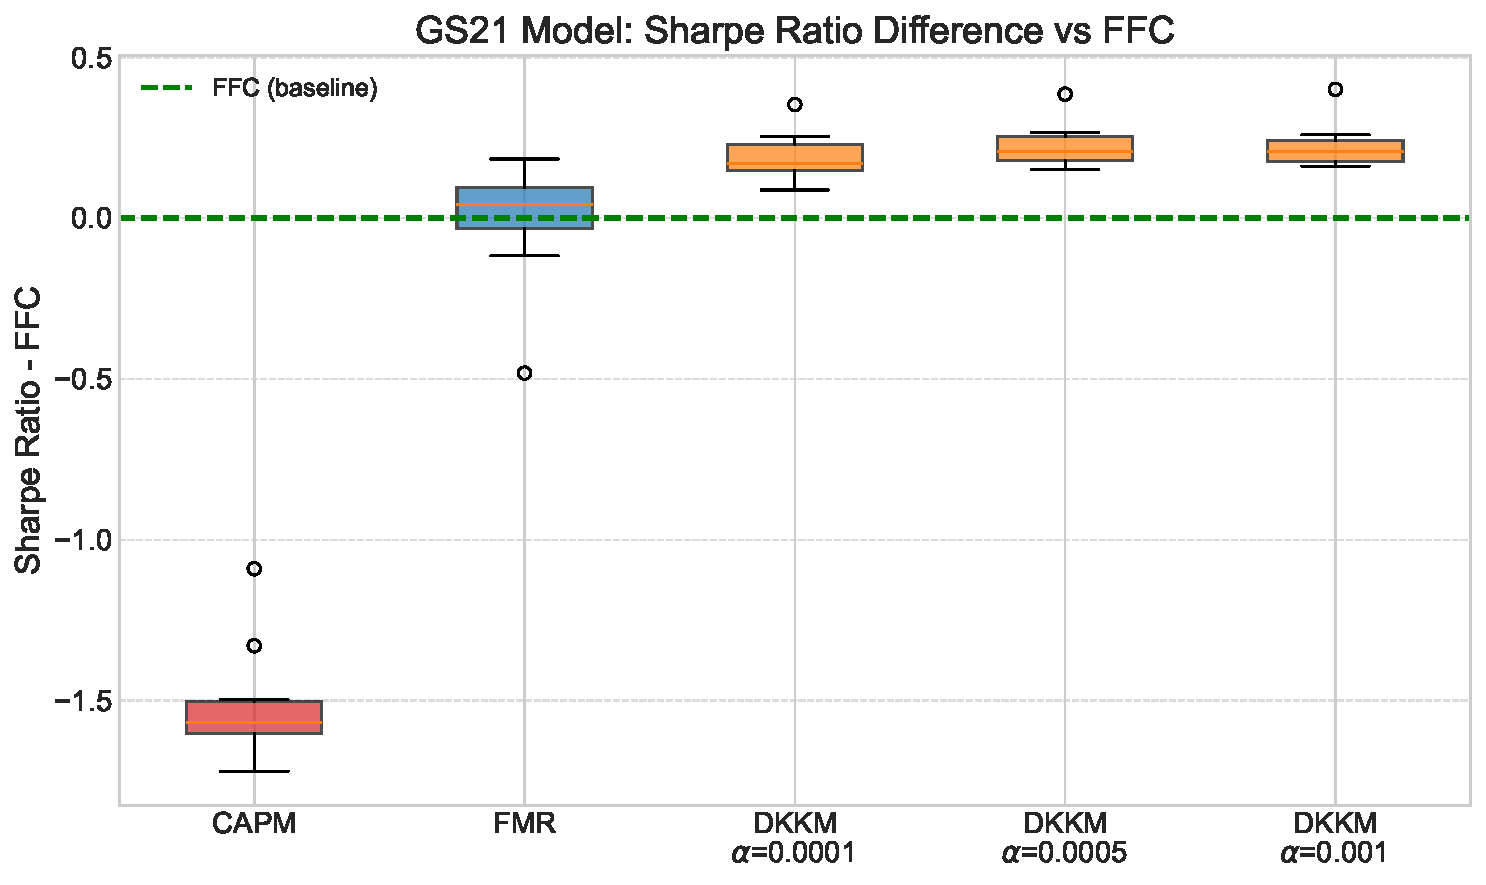
\includegraphics[height=0.85\textheight]{figures/sharpe_boxplot_gs21.pdf}
\end{frame}

\begin{frame}{Statistical Tests: Sharpe Ratios}
DKKM (best $\alpha$, 3600 factors) vs Fama methods

\vspace{0.3cm}
Paired $t$-tests across simulation panels (one-tailed)
  \centering

  \vspace{0.3cm}
  \begin{tabular}{l c c c c c c c c c}
\toprule
& \multicolumn{3}{c}{vs CAPM} & \multicolumn{3}{c}{vs FFC} & \multicolumn{3}{c}{vs FMR} \\
\cmidrule(lr){2-4} \cmidrule(lr){5-7} \cmidrule(lr){8-10}
Model & Diff & $t$ & $p$ & Diff & $t$ & $p$ & Diff & $t$ & $p$ \\
\midrule
BGN & 0.232 & 19.5 & $<$0.001 & 0.067 & 12.6 & $<$0.001 & 0.058 & 9.5 & $<$0.001 \\
KP14 & 0.091 & 29.9 & $<$0.001 & 0.017 & 5.0 & $<$0.001 & 0.026 & 4.6 & $<$0.001 \\
GS21 & 1.751 & 45.4 & $<$0.001 & 0.222 & 11.8 & $<$0.001 & 0.223 & 3.4 & 0.003 \\
\bottomrule
\end{tabular}

  \vspace{0.3cm}
  \raggedright
  \small Positive diff = DKKM has higher Sharpe ratio
\end{frame}

\begin{frame}{Statistical Tests: HJ Distance}
DKKM (best $\alpha$, 3600 factors) vs Fama methods

\vspace{0.3cm}
Paired $t$-tests across simulation panels (one-tailed)
  \centering

  \vspace{0.3cm}
  \begin{tabular}{l c c c c c c c c c}
\toprule
& \multicolumn{3}{c}{vs CAPM} & \multicolumn{3}{c}{vs FFC} & \multicolumn{3}{c}{vs FMR} \\
\cmidrule(lr){2-4} \cmidrule(lr){5-7} \cmidrule(lr){8-10}
Model & Diff & $t$ & $p$ & Diff & $t$ & $p$ & Diff & $t$ & $p$ \\
\midrule
BGN & -0.107 & 4.6 & $<$0.001 & -0.043 & 3.4 & 0.003 & -0.125 & 4.2 & $<$0.001 \\
KP14 & -0.064 & 23.7 & $<$0.001 & -0.023 & 4.7 & $<$0.001 & -0.034 & 6.3 & $<$0.001 \\
GS21 & -0.565 & 25.2 & $<$0.001 & -0.099 & 8.3 & $<$0.001 & -0.132 & 6.5 & $<$0.001 \\
\bottomrule
\end{tabular}

  \vspace{0.3cm}
  \raggedright
  \small Negative diff = DKKM has lower HJ distance (better)
\end{frame}

\begin{frame}{Conclusion}
\begin{itemize}
\item In theoretical economies, we know the true latent SDF, so can calculate the true errors of pricing models.
\item Provides a laboratory for evaluating models
\item Results: DKKM $>$ FFC $\sim$ FMR across all three models
\item All differences statistically significant at $p < 0.01$
\item Next steps: more empirical methods, maybe more theoretical models
\end{itemize}
\end{frame}

\end{document}
